\subsection{Process View}
\subsubsection{Activity Diagrams} \label{seq_diag}

\begin{figure}[h!]
\begin{center}
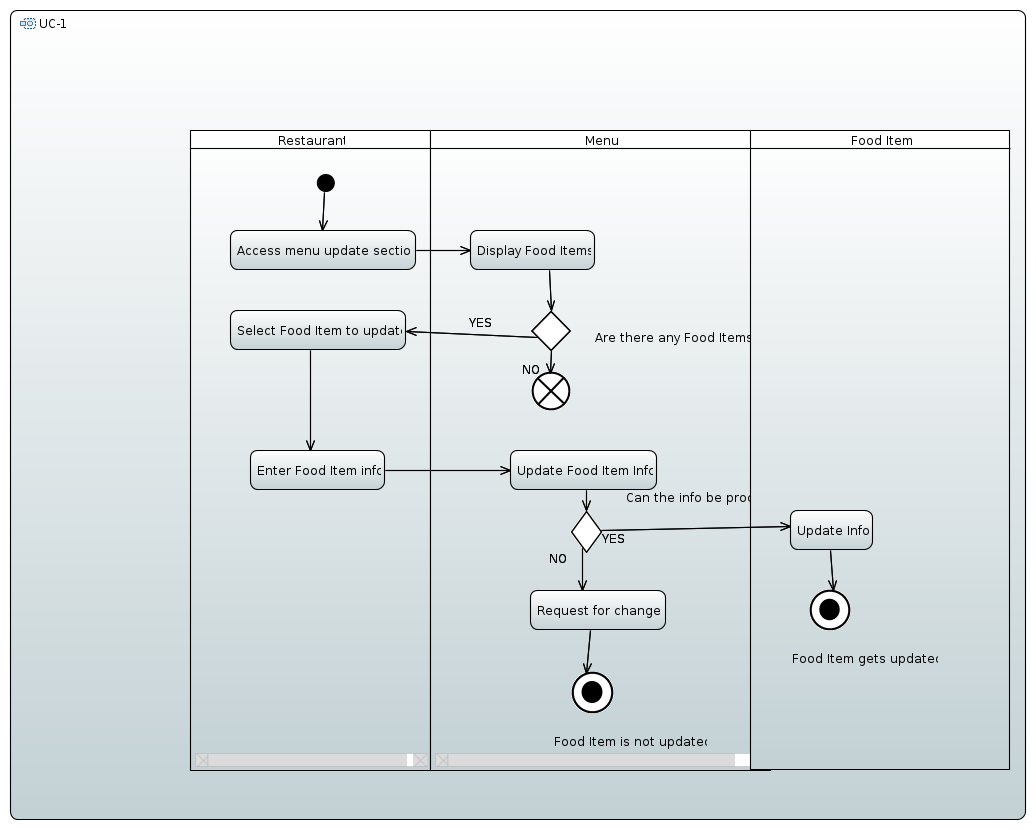
\includegraphics[scale=0.35]{FIGS/UC-1.PNG}
    \caption{Activity Diagram for UC-1}
    \label{fig:act_diag1}
\end{center}
\end{figure}

As described in the first use case, the activity will finish unsuccessfully if there are no food items to update or the provided information is wrong, meaning that it is not supported by the system. Otherwise the activity will finish, successfully updating a food item.

\subsubsection{Sequence Diagram} \label{seq_diag}

\begin{figure}[h!]
\begin{center}
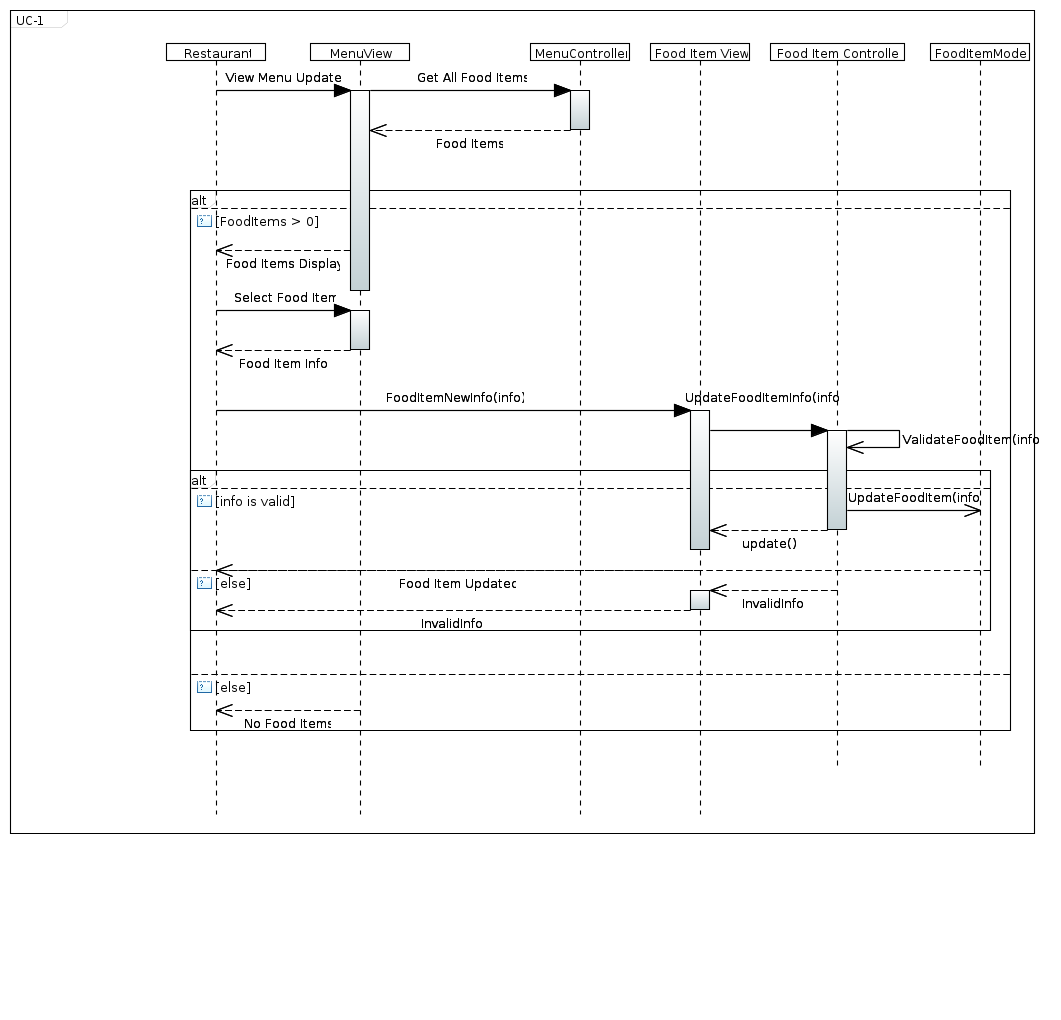
\includegraphics[scale=0.35]{FIGS/UC-11.PNG}
    \caption{Sequence Diagram for UC-1}
    \label{fig:seq_diag1}
\end{center}
\end{figure}

Here the MVC style is considered and the access to the different parts of it controlled. This is, Restaurant can only access the view, not the controller or the model and the model and controller update the view.
